
\section{Implementation}
\label{sec:impl}

The project is divided in two different programs written in C:
one for the neural network learning and the other for the graphical usage.
This approach helps to speed up the learning phase as the viewer executes a
learning update frequency equal to the Frames Per Second (FPS)
(more or less 30).
On the other hand, the dedicated program runs at the effective CPU speed,
executing more than thousands of steps per second.

The learning program is command-line and its synopsis is:
\begin{verbatim}
trainer [-k file] [-c file] [-s file] [-o file] [-r]
\end{verbatim}
where:
\begin{itemize}
    \item \emph{-k} specifies the file describing the Kohonen
             network that is deserialized and serialized at the beginning and
             at the end of the learning process, respectively.
             If the file does not exist or the option is not specified then the
             network is randomly initialized.
             Moreover, the neural network is not serialized if the option is
             not expressed;
    \item \emph{-c} is similar to \emph{-k} but concerns the ACE network;
    \item \emph{-s} is similar to \emph{-k} but concerns the ASE network;
    \item \emph{-o} writes in the specified file the learning advances in a
                    Comma Separated Values (CSV) format;
    \item \emph{-r} starts the learning. Without typing it, the program prints a
                    brief description in order to explain the option meanings
                    and exits.
\end{itemize}
The program execution is ended by sending it a SIGKILL signal (CTRL+C),
causing the neural networks serializations, if possible.

The visualization program uses the neural networks (only Kohonen and ASE)
to show the control usage.
Its synopsis is:
\begin{verbatim}
ball_and_plate [-k file] [-s file] [-r]
\end{verbatim}
where the options have the same meanings.

The graphical program, as shown in Figure~\ref{fig:screenshot}, presents a 
minimalistic layout reporting several basic information and a representation of
the ball and plate system, drawn using the OpenGL library.
The surface within the red boundaries represents the area
in which the controller has to keep the ball to avoid a failure.

\begin{figure}[htb]
  \centering
  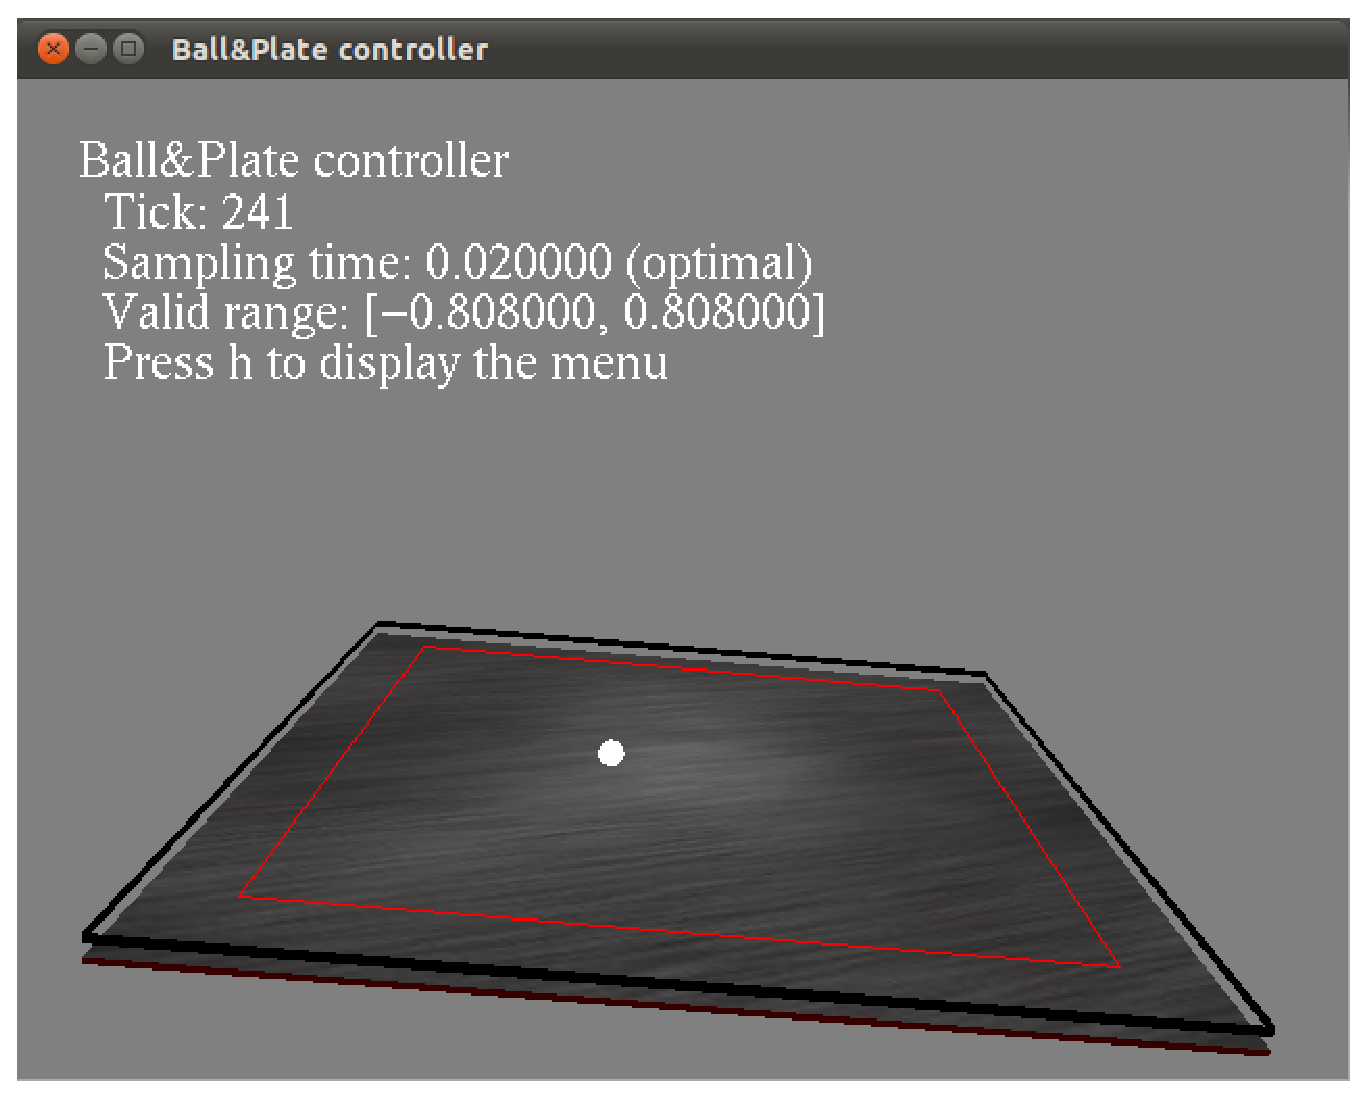
\includegraphics[width=0.9\columnwidth]{screenshot}
  \caption{Program screenshot.}
  \label{fig:screenshot}
\end{figure}

At the top, the program shows the tick number (how many control steps have been
executed), the sampling time (the time elapsed since the last control
event) and the side length of the red boudaries (as percentage of the whole
plate and according to the plate center).

Pressing either \emph{h} or \emph{H} key, the program displays a menu to
explain the available commands.
The keys \emph{w}, \emph{s}, \emph{a} and \emph{d} allow to rotate the 
point of view along the $X$ and $Z$ axis.
To perturbate the system, three features are available.
The \emph{b} key blocks the plate until another press of the same key.
The \emph{directional arrows} let the user to apply an external force to the
ball (not to the plate).
The last feature, enabled by the \emph{c} key, switches between the optimal and
real sampling: with the optimal approach the controller considers a
deterministic sampling every $\Delta t$ (the same used for the learning) while,
with real sampling, the controller works with the actual time elapsed since
the last screen refresh.
The last configuration depends on the graphical capability of the host machine
and the real sampling time usually lasts longer than the optimal one
causing a performance degradation so significant to make the controller
ineffective.
Finally, the \emph{p} and \emph{r} keys pause and reset the simulation,
respectively.

In order to simplify the programs invocations, two scripts are provided: 
\emph{trainer.sh} and \emph{ball\_and\_plate.sh}. Their task is to invoke the
relative programs passing them the pre-trained neural networks files.

% end section

